\documentclass[10pt]{article}
\usepackage{icmlko}

\icmlmeta{IP 파운데이션 월드모델}{139}{풀링은 지켜 주고 희석한다}{노트 138이 던진 질문 --- 웹툰에서 축 다섯이 플래그 하나에 지는 이유. 답은 축이 나빠서가 아니라 풀링이 값을 두 방향으로 쓰기 때문이었다}

\begin{document}

\twocolumn[
\icmlheader

\begin{abstract}
노트 138에서 웹툰의 ``완결인가'' 플래그 하나($+$0.319)가 손으로 매긴 축
다섯의 풀링 모형($+$0.202)을 이겼다. 축이 그 정보를 못 담아서라고 짐작했는데
\textbf{담고 있었다} --- \texttt{entry\_friction}이 완결 플래그와 상관
$-$0.841이고, 웹툰 단독으로 그 축 \emph{하나만} 쓰면 $+$0.3009로 플래그와
사실상 같다. 그러면 왜 다섯을 다 쓰면 지는가. 갈라 보니 웹툰 단독에서
다섯을 다 쓰면 \textbf{$-$0.1907}로 부호가 뒤집힌다. 한 축을 빼면
$+$0.2459로 돌아온다 --- \texttt{goods\_scale}이다. \textbf{여기서 한 번
성급했다.} ``goods\_scale은 독''이라 읽었는데, 전 도메인 풀링에서 그것을
빼 보니 판이 $-$0.027 내리고 게임이 $-$0.252, 아이돌이 $-$0.168 무너진다.
웹툰만 $+$0.021이다. \textbf{풀링 모형에서는 이미 중화돼 있었다.}
그래서 답은 이렇게 정리된다. 풀링은 웹툰에 두 가지를 한다 --- 단독의
$-$0.191을 $+$0.202로 끌어올리는 \textbf{보호}($+$0.393)와, 최선의 단독
$+$0.301을 $+$0.202로 끌어내리는 \textbf{희석}($-$0.099)이다. 희석을
되찾으려면 도메인마다 쓸 축을 고르면 되겠다 싶어 안쪽 분할로 골라 봤다.
\textbf{안 된다.} 웹툰에서 \texttt{goods\_scale}은 안쪽 창 1위($+$0.486)
이면서 바깥 꼴찌($-$0.283)다. 도메인 여섯에서 안쪽 축순위와 바깥 축순위의
상관이 중앙 $+$0.20이고 \textbf{절반이 음수}이며, 둘(웹툰 · 게임)에서는
안쪽 1위가 바깥 꼴찌다.
\end{abstract}
]

\begin{figure*}[t]
\centering
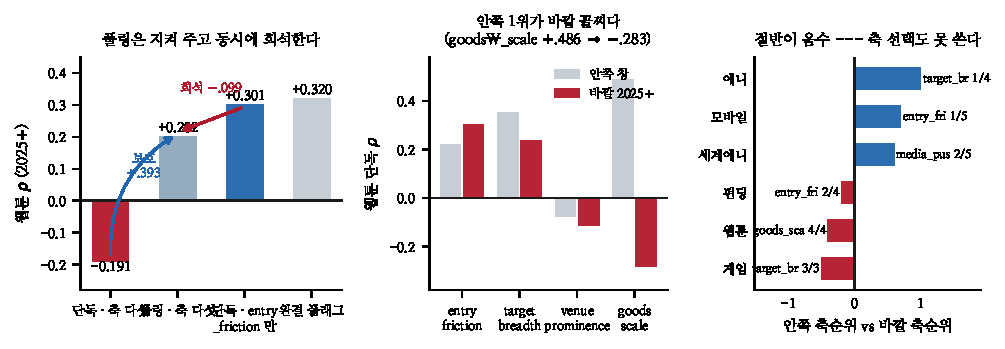
\includegraphics[width=\textwidth]{figs/dilute.pdf}
\caption{왼쪽 --- 풀링의 보호와 희석. 가운데 --- 웹툰에서 안쪽 1위 축이
바깥 꼴찌다. 오른쪽 --- 도메인 여섯 중 셋에서 안-밖 축순위가 음의 상관.}
\end{figure*}

\section{축은 정보를 담고 있었다}

노트 138의 질문은 ``축 다섯이 왜 플래그 하나에 지는가''였고, 가장 단순한
가설은 ``축이 완결 여부를 못 담아서''였다. 틀렸다.

\begin{table}[t]
\centering\tsize
\caption{웹툰 축과 완결 플래그의 상관.}
\begin{tabular}{lrr}
\toprule
& 라벨과 & 완결과 \\
\midrule
\textbf{entry\_friction} & $+$.019 & \textbf{$-$.841} \\
goods\_scale & $+$.033 & $-$.565 \\
target\_breadth & $+$.245 & $-$.287 \\
venue\_prominence & $-$.063 & $-$.104 \\
\bottomrule
\end{tabular}
\end{table}

\claimx{\textbf{\texttt{entry\_friction}은 사실상 완결 플래그다} --- 상관
$-$0.841. 웹툰 단독으로 그 축 하나만 쓰면 $+$0.3009이고 플래그
$+$0.3195와 거의 같다.}{두 축의 상관이 높다는 것이 ``같은 것을 잰다''는
뜻은 아니다. 다만 예측에서 같은 값을 낸다.}

\section{다섯을 다 쓰면 뒤집힌다}

\begin{table}[t]
\centering\tsize
\caption{웹툰 단독 (2025 이전 $\to$ 이후).}
\begin{tabular}{lr}
\toprule
축 하나: entry\_friction & $+$.3009 \\
축 하나: target\_breadth & $+$.2354 \\
축 하나: venue\_prominence & $-$.1124 \\
축 하나: \textbf{goods\_scale} & \textbf{$-$.2827} \\
\midrule
축 다섯 전부 & \textbf{$-$.1907} \\
goods\_scale 뺀 넷 & $+$.2459 \\
\bottomrule
\end{tabular}
\end{table}

한 축을 넣고 빼는 것만으로 $+$0.246과 $-$0.191을 오간다.

\section{그런데 그것을 빼면 판이 내린다}

``\texttt{goods\_scale}은 독''으로 읽고 전 도메인에서 빼 봤다.

\begin{table}[t]
\centering\tsize
\caption{F8 부스팅 · 기본 축. \texttt{goods\_scale}을 뺐을 때의 변화.}
\begin{tabular}{lr}
\toprule
게임 & $-$.252 \\
아이돌 & $-$.168 \\
도서 & $-$.081 \\
팝업 & $-$.037 \\
모바일 · 애니 · 세계애니 & $-$.012 $\sim$ $+$.000 \\
펀딩 & $+$.006 \\
웹툰 & $+$.021 \\
\midrule
\textbf{판} & \textbf{$-$.027} \\
\bottomrule
\end{tabular}
\end{table}

\claimx{\textbf{풀링 모형에서는 이미 중화돼 있었다.} 웹툰 단독에서 $+$0.437을
쥐고 흔들던 축이 풀링에서는 웹툰에 $+$0.021밖에 안 준다. 그리고 게임과
아이돌에서는 크게 값진다. \textbf{빼면 안 된다.}}{``독''이라는 읽기가
성급했다 --- 웹툰 단독이라는 좁은 판에서 본 것을 전 판으로 옮겼다.}

\section{보호와 희석}

\begin{table}[t]
\centering\tsize
\caption{웹툰 $\rho$ (2025$+$). 같은 축, 같은 검정 집합.}
\begin{tabular}{lr}
\toprule
단독 · 축 다섯 & $-$.191 \\
\textbf{풀링 · 축 다섯} & \textbf{$+$.202} \\
단독 · entry\_friction 만 & $+$.301 \\
완결 플래그 & $+$.319 \\
\bottomrule
\end{tabular}
\end{table}

\claimx{\textbf{풀링은 웹툰에 두 가지를 동시에 한다.} 단독의 $-$0.191을
$+$0.202로 끌어올리는 \emph{보호}($+$0.393)와, 최선의 단독 $+$0.301을
$+$0.202로 끌어내리는 \emph{희석}($-$0.099)이다. 노트 126은 보호만
보았고, 희석은 이번에 처음 값으로 잡혔다.}{웹툰 한 도메인의 값이다.
다른 도메인에서는 보호가 없을 수도 희석이 클 수도 있다.}

\section{희석을 되찾으려 했다 --- 안 된다}

계수를 도메인마다 두는 것은 노트 132에서 실패했다(F16). 이번에는 더 낮은
자유도를 시도했다 --- 계수가 아니라 \textbf{쓸 축의 선택}만 도메인마다
바꾼다. 선택은 노트 126의 교훈대로 학습 기간 안쪽 창에서만 한다.

\begin{table}[t]
\centering\tsize
\caption{웹툰 · 축 하나씩. 안쪽은 겹치지 않는 창 다섯의 평균.}
\begin{tabular}{lrr}
\toprule
& 안쪽 & 바깥 (2025$+$) \\
\midrule
\textbf{goods\_scale} & \textbf{$+$.486} & \textbf{$-$.283} \\
target\_breadth & $+$.351 & $+$.235 \\
entry\_friction & $+$.219 & $+$.301 \\
venue\_prominence & $-$.076 & $-$.112 \\
\bottomrule
\end{tabular}
\end{table}

\claimx{\textbf{안쪽 1위가 바깥 꼴찌다.} 웹툰에서 \texttt{goods\_scale}이
안쪽 창 $+$0.486으로 1위이고 바깥에서 $-$0.283으로 꼴찌다. 안쪽 분할로
축을 고르면 정확히 틀린 것을 집는다.}{안쪽 창 다섯의 평균이라 한 창의
잡음은 아니다. 관계가 실제로 뒤집힌 것이다.}

\begin{table}[t]
\centering\tsize
\caption{도메인별 안쪽 축순위 대 바깥 축순위.}
\begin{tabular}{lrrl}
\toprule
& 축 & 순위 상관 & 안쪽 1위의 바깥 순위 \\
\midrule
애니 & 4 & $+$1.00 & 1/4 \\
모바일 & 5 & $+$0.70 & 1/5 \\
세계애니 & 5 & $+$0.60 & 2/5 \\
펀딩 & 4 & $-$0.20 & 2/4 \\
\textbf{웹툰} & 4 & $-$0.40 & \textbf{4/4} \\
\textbf{게임} & 3 & $-$0.50 & \textbf{3/3} \\
\bottomrule
\end{tabular}
\end{table}

\claimx{\textbf{도메인별 축 선택은 못 쓴다.} 안-밖 순위 상관이 중앙
$+$0.20이고 여섯 중 셋이 음수다. 둘에서는 안쪽 1위가 바깥 꼴찌다.
계수든 선택이든, 도메인마다 정하는 것은 안쪽 창으로 검증되지
않는다.}{반대로 애니와 모바일에서는 안쪽이 바깥을 잘 맞힌다($+$1.00 ·
$+$0.70). 도메인마다 ``안쪽을 믿어도 되는가''가 다른데, 그걸 미리 아는
방법이 없다.}

\section{남은 것}

\begin{table}[t]
\centering\tsize
\caption{다음.}
\begin{tabular}{ll}
\toprule
희석 & 값으로 잡혔다($-$0.099). 되찾을 길은 아직 없다 \\
축 정의 & entry\_friction 이 완결 플래그와 $-$0.84 인 것 \\
안쪽 신뢰 & 도메인마다 다른데 미리 아는 법이 없다 \\
\bottomrule
\end{tabular}
\end{table}

둘째 줄이 새 질문이다. \texttt{entry\_friction}은 ``입장 마찰''이고 웹툰에
매길 때 무료 공개인지 유료 회차인지로 읽었을 것이다. 그것이 완결 여부와
$-$0.84로 붙는다는 것은 \textbf{축 정의가 웹툰에서 원래 뜻과 다른 것을
재고 있다}는 뜻이다. 축 이름이 도메인을 건너 같은 뜻을 유지하는지는
노트 5 이후 한 번도 안 재 봤다.

\end{document}
